\documentclass[11pt]{article}
\usepackage{textcomp}
\usepackage{fontenc}

\usepackage{graphicx}
\usepackage{caption}
\usepackage{sidecap}
\usepackage{enumitem}
\usepackage{multicol}
\usepackage{gensymb}
\setlength{\parskip}{3 mm}

\graphicspath{{images/}}	% Root directory of the figures

\title{Interactive Effects of Photoperiod, Temperature, and Chilling on Phenology Across Latitudes}

\renewcommand*{\familydefault}{\sfdefault}



\begin{document}

\maketitle
\section{Abstract}

Woody plant spring phenology drives global carbon cycles and local ecosystem properties. Understanding the sensitivity of forest plants at the species level to abiotic drivers of plant phenology is thus critical for developing predictions of community and ecosystem-level properties. While observational studies of long-term trends are essential for understanding how climate affects timing of phenological events, experimental manipulations can disentangle otherwise covarying environmental factors and directly assess species- and individual-level responses to climate change factors.
Here we present results from a chilling x photoperiod x warming experiment with dormant clippings taken from two different latitudes (42.5 N and 46 N) to address how these interactive effects drive spring leafout phenology across 28 North American woody species. We found photoperiod sensitivity is common in northeastern woody plants and phenological sensitivity to photoperiod and temperature appears largely coordinated across species (i.e., species highly sensitive to temperature were also highly sensitive to photoperiod). Effects of chilling at 1.5 C were less pronounced than effects at 4 C. Overall, however, initial analyses suggest a small role for site (latitude) and chilling in affecting spring phenology. Shrub and small tree species were more sensitive to warming and thus may be more opportunistic with novel climate conditions. In contrast, larger tree species, being less sensitive to temperature cues, may be challenged.

\section{Introduction}


Woody plant spring phenology drives global carbon cycles and local ecosystem properties. Understanding the sensitivity of forest plants at the species level to abiotic drivers of plant phenology is thus critical for developing predictions of community and ecosystem-level properties. 

While observational studies of long-term trends are essential for understanding how climate affects timing of phenological events, experimental manipulations can disentangle otherwise covarying environmental factors and directly assess species- and individual-level responses to climate change factors. 

Here we ask the following questions:
\begin{itemize}
\item{For a suite of northeastern woody plants, what is the role of photoperiod versus temperature in determining timing of budburst, leaf-out, and flowering? Are species limited by photoperiod requirements in their response to warming temperatures?}
\item{To what extent do winter chilling requirements act as additional conservative strategy to avoid damage from early spring freezing?}
\item{Do populations at northern sites, with more severe winters and shorter winter daylength, exhibit more conservative phenological strategies?}
\end{itemize}


Dormancy notes
Conflicting role of photoperiod in tree phenology 
Depending on phenological stage, species and location (Heide 1993; Kramer 1994; Falusi and Calamassi 1996). 
From Chine et al. 2013 book chapter:
long photoperiod enhances cell growth, compensating for a lack of chilling during the endodormancy phase (Wareing 1953; Heide 1993b; Myking and Heide 1995; Caffarra et al. 2011a).

Hanninen divided into sequental and parallel, Chuine 2000 unified.

\section{Materials and Methods}

To test effects of temperature and photoperiod
Woody plant cuttings were made in January 2015 for 28 species which occurred in both Harvard Forest (HF, 42.5\degree N, 72.2\degree W) and the Station de Biologie des Laurentides in St-Hippolyte, Quebec (SH, 45.9\degree N, 74.0\degree W). Cuttings were grown in growth chambers at the Arnold Arboretum in Boston, MA, in distilled water, with water changed every 7-10 days. Cuttings of an individual tree were exposed to each of 12 experimental treatments in a fully-factorial design: 2 temperature (20\degree C / 10\degree C warm vs. 15\degree C / 5\degree C cool) x 2 photoperiod (12 vs. 8 h) x 3 chilling (zero,  33 d at 4\degree C, 33 d at 1.5\degree C) treatments. 

With 6 replicates of these species across 6 experimental treatments being monitored at 5-7 day intervals for over 3 months, we made over 17,500 individual phenological observations following a modified BBCH scale.


\section{Results}

Temperature and photoperiod individually and interactively determined timing of leaf-out, with strongest effects of temperature in short-day conditions. A literature review found 42 studies which investigated effects of photoperiod, temperature, or their interaction on the timing of bud burst or flowering for woody or semi-woody plants.  No study varied chilling period, photoperiod, and temperature simultaneously across species. We found increasing photoperiod significantly reduced time to phenological responses for a portion of studies, but effects strongly depended on taxa examined. Figure 1 summarizes overall effects of temperature and daylength across latitudes, showing greater effect of warming in short-day conditions.

Species-specific sensitivity to temperature and photoperiod as cues for leaf-out times, as estimated by mixed-effect model. Sensitivity to temperature and photoperiod manipulations are largely coordinated, with shrubs and small trees advanced in leaf-out (negative responses) by both factors.

Table  summarizes a mixed-effects model analysis of leaf-out day, with negative values indicate earlier leaf-out day of experiment. With species as random effects, overall the 5\degree C experimental warming resulted in over 14 days earlier warming; such advance was delayed by the severe chilling treatment. Latitude of origin overall had little direct effect on leaf-out, but populations from the northern site did exhibit more rapid leaf-out under the severe chilling treatment.

Species varied widely in response to chilling treatments, with some exhibiting strong chilling requirements (\emph{Acer saccharum}, \emph{Fagus grandifolia}), while others exhibited little change in phenological advacement under experimentally manipulated chilling. Overall, leaf-out was advanced by 4.5 days under additional 30 d of vernalization at 4\degree C, and non-significantly delayed 0.67 days under additional 30 d of vernalization at 1.5\degree C.

Response of \emph{Fagus grandifolia} to increasingly strong vernalization varies by latitude of origin and by phenological stage; winter chilling reduced day to budburst (right) and leaf-out (left), but more strongly for individuals from the northern SH site.


% from Pheno budburst analyses.R, using memisc and xtable

Warming, photoperiod, and chilling individually and interactively acted to drive budburst  and leafout earlier across species. The strength of the accelleration in budburst due to both warming and photoperiod were similar, but the accelleration of leafout due to warming exceeded that of photoperiod. Surprisingly, site of origin exerted no effect on either budburst or leafout across species.

Table 1. Summary of mixed effect model of budburst day by species

\begin{table}[ht]
\centering
\begin{tabular}{rrrrrrr}
  \hline
 & est & se & stat & p & lwr & upr \\ 
  \hline
(Intercept) & 25.90 & 1.75 & 14.76 & 0.00 & 22.46 & 29.34 \\ 
  warmn & -2.20 & 0.43 & -5.16 & 0.00 & -3.03 & -1.36 \\ 
  photon & -2.50 & 0.39 & -6.34 & 0.00 & -3.27 & -1.73 \\ 
  siteSH & -0.41 & 0.43 & -0.96 & 0.34 & -1.24 & 0.43 \\ 
  chilln & -3.99 & 0.33 & -11.93 & 0.00 & -4.65 & -3.34 \\ 
  warmn:photon & -0.20 & 0.28 & -0.73 & 0.46 & -0.75 & 0.34 \\ 
  warmn:siteSH & -0.49 & 0.41 & -1.18 & 0.24 & -1.29 & 0.32 \\ 
  photon:siteSH & 0.06 & 0.41 & 0.14 & 0.89 & -0.75 & 0.87 \\ 
  warmn:chilln & 2.16 & 0.30 & 7.16 & 0.00 & 1.57 & 2.75 \\ 
  photon:chilln & -0.11 & 0.31 & -0.34 & 0.73 & -0.71 & 0.50 \\ 
  siteSH:chilln & -0.52 & 0.44 & -1.18 & 0.24 & -1.37 & 0.34 \\ 
  warmn:photon:siteSH & -0.13 & 0.41 & -0.32 & 0.75 & -0.93 & 0.67 \\ 
  warmn:photon:chilln & -0.59 & 0.29 & -2.02 & 0.04 & -1.17 & -0.02 \\ 
  warmn:siteSH:chilln & -0.31 & 0.42 & -0.74 & 0.46 & -1.14 & 0.51 \\ 
  photon:siteSH:chilln & 0.06 & 0.42 & 0.15 & 0.88 & -0.77 & 0.89 \\ 
  warmn:photon:siteSH:chilln & 0.06 & 0.42 & 0.14 & 0.89 & -0.77 & 0.88 \\ 
           Var(\~{}1$|$sp) & 60.41 &  &  &  &  &  \\ 
       Var(\~{}warmn$|$sp) & 2.72 &  &  &  &  &  \\ 
     Cov(\~{}1:warmn$|$sp) & -12.82 &  &  &  &  &  \\ 
         Var(\~{}1$|$sp.1) & 22.57 &  &  &  &  &  \\ 
    Var(\~{}photon$|$sp.1) & 1.88 &  &  &  &  &  \\ 
  Cov(\~{}1:photon$|$sp.1) & -6.52 &  &  &  &  &  \\ 
        Var(residual) & 68.42 &  &  &  &  &  \\ 
   \hline
\end{tabular}
\end{table}

Table 2. Summary of mixed effect model of leafout day by species.

\begin{table}[ht]
\centering
\begin{tabular}{rrrrrrr}
  \hline
 & est & se & stat & p & lwr & upr \\ 
  \hline
(Intercept) & 38.24 & 1.99 & 19.22 & 0.00 & 34.34 & 42.14 \\ 
  warmn & -5.50 & 0.76 & -7.21 & 0.00 & -7.00 & -4.01 \\ 
  photon & -3.78 & 0.70 & -5.38 & 0.00 & -5.16 & -2.40 \\ 
  site & 0.29 & 0.46 & 0.63 & 0.53 & -0.61 & 1.18 \\ 
  chilln & -3.83 & 0.76 & -5.07 & 0.00 & -5.32 & -2.35 \\ 
  warmn:photon & 0.98 & 0.68 & 1.45 & 0.15 & -0.34 & 2.30 \\ 
  warmn:site & -0.44 & 0.44 & -1.00 & 0.32 & -1.30 & 0.42 \\ 
  photon:site & -0.46 & 0.44 & -1.04 & 0.30 & -1.32 & 0.41 \\ 
  warmn:chilln & 3.72 & 0.71 & 5.23 & 0.00 & 2.33 & 5.12 \\ 
  photon:chilln & 1.21 & 0.71 & 1.69 & 0.09 & -0.19 & 2.61 \\ 
  site:chilln & -0.43 & 0.46 & -0.92 & 0.36 & -1.34 & 0.49 \\ 
  warmn:photon:site & -0.13 & 0.44 & -0.30 & 0.76 & -0.99 & 0.72 \\ 
  warmn:photon:chilln & -1.63 & 0.70 & -2.31 & 0.02 & -3.01 & -0.25 \\ 
  warmn:site:chilln & -0.75 & 0.45 & -1.66 & 0.10 & -1.63 & 0.13 \\ 
  photon:site:chilln & -0.45 & 0.45 & -1.01 & 0.31 & -1.34 & 0.43 \\ 
  warmn:photon:site:chilln & 0.40 & 0.45 & 0.89 & 0.37 & -0.48 & 1.28 \\ 
           Var(\~{}1$|$sp) & 80.60 &  &  &  &  &  \\ 
       Var(\~{}warmn$|$sp) & 3.40 &  &  &  &  &  \\ 
     Cov(\~{}1:warmn$|$sp) & -16.57 &  &  &  &  &  \\ 
         Var(\~{}1$|$sp.1) & 16.75 &  &  &  &  &  \\ 
    Var(\~{}photon$|$sp.1) & 0.95 &  &  &  &  &  \\ 
  Cov(\~{}1:photon$|$sp.1) & -3.99 &  &  &  &  &  \\ 
        Var(residual) & 78.07 &  &  &  &  &  \\ 
   \hline
\end{tabular}
\end{table}

%%%%%%%%%%% Figures for these tables
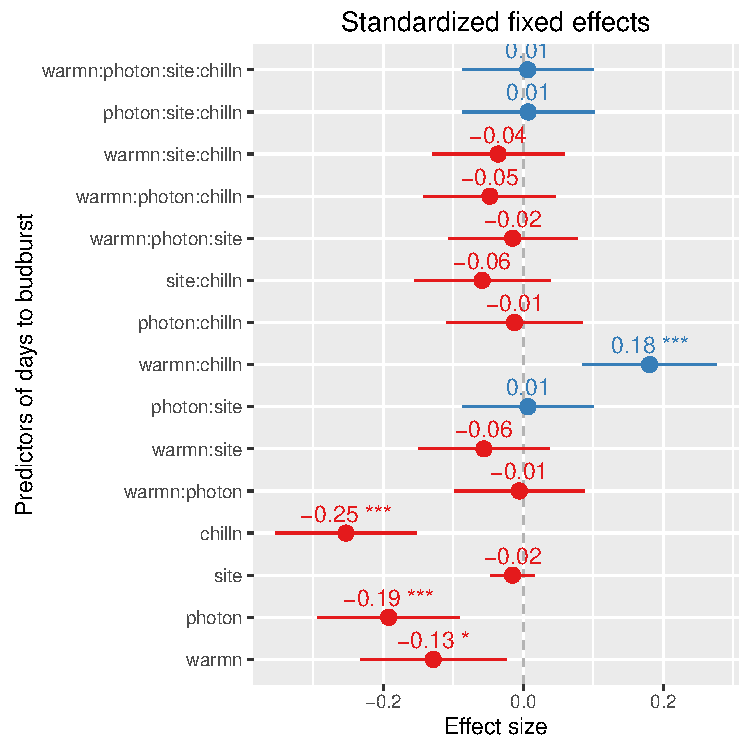
\includegraphics[scale=0.5]{lmerDBB}


Species traits partly explain variation in budburst and leafout. Plant with high nitrogen leaves, as well as high SLA (thinner, less dense) leaves, were significantly later in both budburst and leafout. Thus early leafout species tended to be tougher, less N-dense, and have higher carbon investments than later species. Greater wood density

Ring-porous species (Fraxinus sp., Lonicera, Myrica, and Quercus; lower values of Pore Anatomy variable) exhibited significantly later budburst and leafout compared to diffuse-porous species, in line with previous work on wood anatomy and freezing risk (Sperrry \& Sullivan 1991 Plant Phys).


Table 3. Summary of species-specific predictors of budburst day. 
\begin{table}[ht]
\centering
\begin{tabular}{rrrrrrr}
  \hline
 & est & se & stat & p & lwr & upr \\ 
  \hline
Intercept & 26.48 & 0.30 & 88.55 & 0.00 & 25.90 & 27.07 \\ 
  Wood density & 2.02 & 0.36 & 5.65 & 0.00 & 1.32 & 2.73 \\ 
  SLA & 2.18 & 0.30 & 7.21 & 0.00 & 1.59 & 2.78 \\ 
  \% N & 4.00 & 0.34 & 11.61 & 0.00 & 3.32 & 4.67 \\ 
  Pore Anatomy & -3.69 & 0.31 & -11.82 & 0.00 & -4.30 & -3.08 \\ 
   \hline
\end{tabular}
\end{table}

Table 4. Summary of species-specific predictors of leafout day. 
\begin{table}[ht]
\centering
\begin{tabular}{rrrrrrr}
  \hline
 & est & se & stat & p & lwr & upr \\ 
  \hline
 Intercept & 37.44 & 0.37 & 102.24 & 0.00 & 36.72 & 38.15 \\ 
  Wood density & -0.18 & 0.46 & -0.38 & 0.70 & -1.08 & 0.73 \\ 
  SLA & 1.83 & 0.37 & 4.95 & 0.00 & 1.11 & 2.56 \\ 
  \% N & 3.97 & 0.43 & 9.28 & 0.00 & 3.13 & 4.81 \\ 
Pore Anatomy & -0.89 & 0.38 & -2.36 & 0.02 & -1.63 & -0.15 \\ 
   \hline
\end{tabular}
\end{table}


Table 5. Phylogenetic signal in timing of budburst and leafout and species specific traits. 

\begin{table}[ht]
\centering
\begin{tabular}{rlrrr}
  \hline
 & Variable & K & PIC variance & PIC variance P \\ 
  \hline
1 & Budburst & 0.02 & 47.53 & 0.73 \\ 
  2 & Leafout & 0.03 & 38.47 & 0.58 \\ 
  3 & Wood Density & 0.25 & 0.04 & 0.06 \\ 
  4 & Pore anatomy & 1.38 & 0.01 & 0.00 \\ 
  5 & SLA & 0.15 & 240.79 & 0.19 \\ 
  6 & \% N & 0.19 & 0.01 & 0.12 \\ 
   \hline
\end{tabular}
\end{table}


\subsection{Nonleafouts}

Separate analysis of samples which did not break bud or leafout. Across species, there was no overall predictive effect of temperature, photoperiod, chilling, or site on the propensity to fail to leaf out. 
Species ranged from complete leafout (Hamammaelis) to only 50\% leafout (Fagus grandifolia, Acer saccharum) across all treatments. The percent of nonleafout s by site was similar, with 12.4\% of Harvard Forest and 9.5\% of St. Hippolyte samples failing to leaf out. Examining individual species,  there was an interaction of temperatuer by daylength for some species, with greater failure to leafout in cool, short conditions for Acer pensylvanicum  and Acer saccharum (chi-sq, glm results). Site effects were in consistent, with greater failure to leafout for cuttings from St. Hippolyte in Acer rubrum and Fagus grandifolia, and from Harvard Forest in Acer saccharum (glm results).
 
\subsection{Leafout by day of year method}


 

\section{Discussion}

\begin{itemize}

\item{Photoperiod sensitivity is common in northeastern woody plants; Phenological sensitivity to photoperiod and temperature are largely coordinated across species.}
\item{Under warming climates, shrubs and small trees are more opportunistic with novel climate conditions. Larger trees, being less sensitive to temperature cues, will be challenged. }
\item{Initial analysis shows little increase in risk-avoidance strategies for northern populations of these 28 species}
\item{Future work will integrate bud and wood anatomy and leaf functional traits to develop species-level predictions of northeastern forest phenological change under future climate conditions.}
\end{itemize}


\section{Supplemental Figures and Tables}

% Stan output for budburst day of year model

Supplemental Table 2. Stan output for analysis of leafout day by species and site. Parameters for site (a1 and a2) and species-level parameters for effects of warming (b_warm), photoperiod (b_photo), chilling (b_chill), and the interaction of warming and photoperiod (b_inter) shown.

\begin{table}[ht]
\centering
\begin{tabular}{rrrrrrrrrrr}
  \hline
 & mean & se\_mean & sd & 2.5\% & 25\% & 50\% & 75\% & 97.5\% & n\_eff & Rhat \\ 
  \hline
a[1] & 37.84 & 5.59 & 7.91 & 28.28 & 31.26 & 37.45 & 44.14 & 48.09 & 2.00 & 275.21 \\ 
  a[2] & 36.05 & 5.16 & 7.30 & 24.73 & 32.80 & 37.34 & 40.57 & 44.83 & 2.00 & 387.34 \\ 
  b\_warm[1] & -4.16 & 3.62 & 5.12 & -9.27 & -6.98 & -6.15 & -2.80 & 4.49 & 2.00 & 60.99 \\ 
  b\_warm[2] & 3.61 & 1.13 & 1.61 & 1.34 & 2.47 & 3.67 & 5.34 & 5.56 & 2.01 & 25.28 \\ 
  b\_warm[3] & 9.34 & 2.29 & 3.25 & 4.41 & 7.13 & 10.36 & 12.18 & 12.54 & 2.00 & 42.12 \\ 
  b\_warm[4] & -3.42 & 4.14 & 5.87 & -13.56 & -4.22 & -1.03 & -0.04 & 2.03 & 2.00 & 43.76 \\ 
  b\_warm[5] & -8.79 & 3.59 & 5.08 & -12.79 & -12.30 & -11.10 & -7.71 & -0.09 & 2.00 & 109.28 \\ 
  b\_warm[6] & 0.51 & 2.14 & 3.03 & -3.03 & -1.91 & 0.09 & 2.41 & 4.98 & 2.00 & 68.61 \\ 
  b\_warm[7] & -5.48 & 2.60 & 3.69 & -11.05 & -7.44 & -5.04 & -2.74 & -0.99 & 2.00 & 55.68 \\ 
  b\_warm[8] & -1.55 & 2.21 & 3.13 & -6.06 & -2.94 & -1.62 & 0.37 & 2.78 & 2.01 & 37.16 \\ 
  b\_warm[9] & -6.98 & 3.32 & 4.70 & -15.06 & -7.66 & -4.87 & -3.95 & -3.26 & 2.00 & 122.32 \\ 
  b\_warm[10] & 14.94 & 4.19 & 5.93 & 5.23 & 13.36 & 16.57 & 18.07 & 21.58 & 2.00 & 117.63 \\ 
  b\_warm[11] & -5.69 & 1.41 & 1.99 & -8.01 & -6.80 & -6.17 & -5.08 & -2.36 & 2.00 & 36.45 \\ 
  b\_warm[12] & -6.10 & 4.76 & 6.74 & -13.43 & -10.62 & -7.67 & -3.91 & 5.06 & 2.00 & 60.67 \\ 
  b\_warm[13] & -0.19 & 1.88 & 2.66 & -3.95 & -1.56 & -0.40 & 1.38 & 3.72 & 2.01 & 24.32 \\ 
  b\_warm[14] & -4.78 & 1.58 & 2.24 & -7.68 & -5.89 & -5.03 & -3.93 & -1.38 & 2.00 & 103.89 \\ 
  b\_warm[15] & -8.31 & 3.13 & 4.43 & -15.17 & -10.56 & -7.51 & -5.37 & -3.01 & 2.00 & 106.42 \\ 
  b\_warm[16] & -19.45 & 6.31 & 8.93 & -29.20 & -25.39 & -22.31 & -15.94 & -4.85 & 2.00 & 40.02 \\ 
  b\_warm[17] & -6.05 & 1.58 & 2.23 & -7.85 & -7.69 & -7.10 & -5.36 & -2.25 & 2.00 & 42.03 \\ 
  b\_warm[18] & 10.23 & 2.75 & 3.89 & 6.53 & 7.84 & 8.83 & 10.70 & 17.11 & 2.00 & 34.89 \\ 
  b\_warm[19] & -3.57 & 3.22 & 4.55 & -6.85 & -6.24 & -5.83 & -3.37 & 4.53 & 2.00 & 40.37 \\ 
  b\_warm[20] & 4.42 & 6.58 & 9.31 & -10.63 & 0.94 & 7.01 & 10.43 & 14.38 & 2.00 & 360.81 \\ 
  b\_warm[21] & 3.14 & 2.56 & 3.63 & -1.56 & 0.78 & 2.75 & 5.21 & 8.48 & 2.00 & 61.59 \\ 
  b\_warm[22] & 10.77 & 6.15 & 8.71 & -0.70 & 7.14 & 9.97 & 13.57 & 23.86 & 2.00 & 217.57 \\ 
  b\_warm[23] & -10.14 & 3.07 & 4.35 & -16.97 & -12.08 & -9.22 & -7.39 & -4.88 & 2.00 & 42.60 \\ 
  b\_warm[24] & -13.36 & 3.19 & 4.51 & -17.04 & -16.86 & -15.27 & -11.87 & -5.81 & 2.00 & 218.04 \\ 
  b\_warm[25] & -11.62 & 2.50 & 3.53 & -15.46 & -14.39 & -12.48 & -9.43 & -5.99 & 2.00 & 35.96 \\ 
  b\_warm[26] & -7.94 & 3.80 & 5.37 & -13.48 & -12.15 & -9.38 & -5.29 & 1.13 & 2.01 & 34.93 \\ 
  b\_warm[27] & -3.37 & 1.72 & 2.43 & -6.54 & -5.26 & -3.52 & -1.18 & -0.15 & 2.00 & 34.57 \\ 
  b\_warm[28] & -1.15 & 3.44 & 4.87 & -9.49 & -2.76 & 1.04 & 2.04 & 3.13 & 2.00 & 70.82 \\ 
  b\_photo[1] & -8.67 & 2.72 & 3.85 & -13.55 & -11.28 & -9.21 & -6.44 & -2.96 & 2.00 & 78.32 \\ 
  b\_photo[2] & -2.32 & 0.76 & 1.08 & -3.96 & -2.82 & -2.32 & -1.55 & -0.87 & 2.01 & 15.71 \\ 
  b\_photo[3] & 13.75 & 3.80 & 5.38 & 5.56 & 11.32 & 14.43 & 16.91 & 20.55 & 2.00 & 88.11 \\ 
  b\_photo[4] & 0.33 & 2.03 & 2.88 & -3.57 & -1.84 & 0.54 & 2.74 & 3.79 & 2.00 & 69.70 \\ 
  b\_photo[5] & -8.40 & 3.71 & 5.25 & -12.67 & -11.92 & -10.77 & -7.29 & 0.58 & 2.00 & 91.46 \\ 
  b\_photo[6] & -2.53 & 2.55 & 3.60 & -7.18 & -5.30 & -2.60 & 0.09 & 2.30 & 2.00 & 144.63 \\ 
  b\_photo[7] & -1.10 & 3.50 & 4.95 & -8.36 & -3.13 & -0.85 & 1.27 & 5.64 & 2.00 & 124.95 \\ 
  b\_photo[8] & 0.28 & 2.00 & 2.83 & -4.22 & -0.85 & 0.96 & 1.86 & 3.68 & 2.00 & 69.65 \\ 
  b\_photo[9] & -4.79 & 4.08 & 5.77 & -14.83 & -5.29 & -1.77 & -1.35 & -0.81 & 2.00 & 34.92 \\ 
  b\_photo[10] & 3.05 & 2.31 & 3.27 & -0.72 & 0.49 & 2.72 & 4.75 & 8.24 & 2.01 & 23.88 \\ 
  b\_photo[11] & -0.07 & 1.45 & 2.06 & -2.22 & -2.13 & -0.08 & 1.99 & 2.02 & 2.00 & 67.44 \\ 
  b\_photo[12] & -3.44 & 5.97 & 8.45 & -13.73 & -9.43 & -4.77 & 1.19 & 9.31 & 2.00 & 92.41 \\ 
  b\_photo[13] & -3.71 & 2.31 & 3.26 & -6.82 & -6.68 & -4.63 & -1.53 & 1.11 & 2.00 & 140.49 \\ 
  b\_photo[14] & 1.14 & 1.36 & 1.92 & -1.63 & 0.27 & 1.22 & 2.00 & 3.95 & 2.00 & 71.73 \\ 
  b\_photo[15] & -5.15 & 3.19 & 4.53 & -12.04 & -7.21 & -5.49 & -1.80 & 0.60 & 2.01 & 18.21 \\ 
  b\_photo[16] & -12.91 & 5.78 & 8.18 & -21.83 & -17.97 & -15.13 & -9.87 & 0.32 & 2.00 & 230.19 \\ 
  b\_photo[17] & -3.53 & 1.05 & 1.48 & -5.50 & -4.51 & -3.79 & -2.28 & -1.38 & 2.01 & 17.30 \\ 
  b\_photo[18] & 17.44 & 4.84 & 6.85 & 9.38 & 11.35 & 17.22 & 23.52 & 25.82 & 2.00 & 76.36 \\ 
  b\_photo[19] & -3.36 & 3.43 & 4.86 & -10.87 & -5.43 & -2.69 & -0.58 & 2.81 & 2.00 & 85.10 \\ 
  b\_photo[20] & -3.61 & 4.87 & 6.89 & -11.45 & -8.95 & -4.83 & 0.41 & 6.71 & 2.00 & 195.30 \\ 
  b\_photo[21] & 2.49 & 2.45 & 3.47 & -2.37 & 0.78 & 1.92 & 3.89 & 7.95 & 2.01 & 29.85 \\ 
  b\_photo[22] & 21.50 & 4.20 & 5.95 & 12.76 & 18.08 & 21.60 & 25.06 & 29.60 & 2.00 & 56.87 \\ 
  b\_photo[23] & 0.45 & 3.47 & 4.91 & -5.47 & -2.65 & -0.49 & 2.90 & 8.11 & 2.00 & 108.22 \\ 
  b\_photo[24] & 0.01 & 1.31 & 1.86 & -1.95 & -1.73 & -0.37 & 1.46 & 2.75 & 2.01 & 18.71 \\ 
  b\_photo[25] & -8.52 & 2.30 & 3.26 & -13.64 & -10.19 & -7.71 & -5.75 & -5.04 & 2.00 & 44.49 \\ 
  b\_photo[26] & -4.31 & 3.83 & 5.43 & -10.50 & -9.21 & -4.54 & -0.01 & 2.75 & 2.00 & 33.18 \\ 
  b\_photo[27] & -5.89 & 1.96 & 2.77 & -9.93 & -7.33 & -6.04 & -4.16 & -2.04 & 2.00 & 37.54 \\ 
  b\_photo[28] & -0.72 & 2.23 & 3.15 & -6.21 & -1.03 & 0.80 & 1.29 & 1.53 & 2.01 & 34.53 \\ 
  b\_chill[1] & -19.01 & 15.75 & 22.28 & -57.03 & -23.22 & -9.45 & -3.99 & -0.85 & 2.00 & 121.98 \\ 
  b\_chill[2] & -7.83 & 9.12 & 12.90 & -16.79 & -16.29 & -14.47 & -6.13 & 14.49 & 2.00 & 290.40 \\ 
  b\_chill[3] & 7.22 & 27.65 & 39.12 & -21.18 & -17.05 & -12.42 & 12.06 & 74.58 & 2.00 & 762.99 \\ 
  b\_chill[4] & -7.87 & 22.90 & 32.40 & -57.36 & -18.61 & -3.79 & 6.94 & 33.53 & 2.00 & 1223.29 \\ 
  b\_chill[5] & 30.45 & 9.75 & 13.79 & 13.18 & 19.00 & 31.00 & 42.55 & 46.53 & 2.00 & 397.29 \\ 
  b\_chill[6] & -20.17 & 5.70 & 8.06 & -29.02 & -26.87 & -21.71 & -16.20 & -7.45 & 2.00 & 44.63 \\ 
  b\_chill[7] & 37.60 & 17.33 & 24.52 & -3.33 & 32.87 & 44.89 & 51.87 & 62.28 & 2.00 & 112.47 \\ 
  b\_chill[8] & 26.89 & 6.69 & 9.46 & 11.63 & 22.73 & 29.13 & 33.25 & 37.43 & 2.00 & 97.38 \\ 
  b\_chill[9] & 0.71 & 27.29 & 38.62 & -43.71 & -29.78 & -5.16 & 25.74 & 56.67 & 2.00 & 395.18 \\ 
  b\_chill[10] & 5.00 & 24.75 & 35.02 & -48.80 & -14.98 & 14.57 & 36.68 & 36.97 & 2.00 & 86.72 \\ 
  b\_chill[11] & 13.28 & 28.31 & 40.06 & -42.96 & -7.34 & 13.50 & 34.12 & 69.29 & 2.00 & 249.28 \\ 
  b\_chill[12] & 9.56 & 27.86 & 39.42 & -45.96 & -7.34 & 9.79 & 25.81 & 65.52 & 2.00 & 330.48 \\ 
  b\_chill[13] & -14.45 & 22.79 & 32.24 & -47.20 & -41.99 & -22.26 & 5.43 & 33.75 & 2.00 & 364.03 \\ 
  b\_chill[14] & 6.91 & 14.08 & 19.93 & -18.78 & -6.40 & 5.73 & 18.24 & 35.75 & 2.00 & 149.96 \\ 
  b\_chill[15] & -16.14 & 13.90 & 19.67 & -42.56 & -31.10 & -14.56 & 0.30 & 7.06 & 2.00 & 281.61 \\ 
  b\_chill[16] & -14.09 & 32.99 & 46.68 & -90.57 & -32.56 & 4.19 & 22.56 & 25.95 & 2.00 & 2220.83 \\ 
  b\_chill[17] & 14.46 & 19.18 & 27.14 & -22.76 & 1.29 & 13.07 & 27.34 & 53.73 & 2.00 & 126.10 \\ 
  b\_chill[18] & -24.65 & 41.33 & 58.48 & -75.49 & -59.65 & -49.31 & -13.81 & 74.72 & 2.00 & 376.18 \\ 
  b\_chill[19] & -11.09 & 10.64 & 15.06 & -25.77 & -20.99 & -16.29 & -6.47 & 14.16 & 2.00 & 131.17 \\ 
  b\_chill[20] & 4.18 & 23.80 & 33.67 & -38.49 & -11.83 & -0.46 & 15.37 & 56.13 & 2.00 & 224.52 \\ 
  b\_chill[21] & -5.39 & 4.05 & 5.73 & -12.58 & -8.51 & -6.26 & -3.21 & 3.82 & 2.00 & 48.73 \\ 
  b\_chill[22] & 0.02 & 43.15 & 61.05 & -87.20 & -42.26 & 10.15 & 53.08 & 65.79 & 2.00 & 178.85 \\ 
  b\_chill[23] & -13.26 & 29.71 & 42.03 & -71.95 & -35.00 & -13.47 & 8.94 & 45.59 & 2.00 & 387.35 \\ 
  b\_chill[24] & -10.68 & 17.13 & 24.24 & -38.62 & -25.98 & -15.80 & -0.49 & 27.57 & 2.00 & 415.65 \\ 
  b\_chill[25] & 32.12 & 18.95 & 26.81 & -9.90 & 20.40 & 37.89 & 49.04 & 63.13 & 2.00 & 297.00 \\ 
  b\_chill[26] & -13.66 & 9.61 & 13.59 & -30.09 & -25.05 & -14.18 & -2.70 & 3.85 & 2.00 & 173.60 \\ 
  b\_chill[27] & 5.55 & 7.83 & 11.08 & -11.31 & -1.03 & 7.98 & 14.29 & 17.76 & 2.00 & 127.82 \\ 
  b\_chill[28] & -8.77 & 16.82 & 23.80 & -40.78 & -21.41 & -9.95 & 2.43 & 25.99 & 2.00 & 299.61 \\ 
  b\_inter[1] & 1.88 & 2.14 & 3.03 & -3.19 & 0.56 & 3.13 & 4.18 & 4.56 & 2.00 & 56.03 \\ 
  b\_inter[2] & -3.32 & 0.46 & 0.66 & -4.56 & -3.40 & -3.01 & -2.93 & -2.78 & 2.01 & 23.03 \\ 
  b\_inter[3] & -11.93 & 2.65 & 3.75 & -17.95 & -13.37 & -11.01 & -9.66 & -7.64 & 2.00 & 74.98 \\ 
  b\_inter[4] & -3.35 & 2.29 & 3.24 & -5.64 & -5.60 & -4.96 & -2.78 & 2.27 & 2.00 & 123.52 \\ 
  b\_inter[5] & 4.54 & 2.34 & 3.32 & -1.19 & 4.02 & 6.22 & 6.63 & 7.09 & 2.00 & 71.74 \\ 
  b\_inter[6] & -1.46 & 1.47 & 2.08 & -4.31 & -3.05 & -1.37 & 0.21 & 1.20 & 2.00 & 64.95 \\ 
  b\_inter[7] & -0.87 & 2.65 & 3.75 & -6.89 & -2.15 & -0.23 & 1.45 & 3.48 & 2.01 & 40.44 \\ 
  b\_inter[8] & -1.20 & 1.16 & 1.64 & -3.49 & -1.98 & -1.21 & -0.56 & 1.18 & 2.00 & 52.03 \\ 
  b\_inter[9] & -0.07 & 2.36 & 3.34 & -3.42 & -1.81 & -1.22 & 0.49 & 5.58 & 2.00 & 68.91 \\ 
  b\_inter[10] & -11.07 & 1.76 & 2.49 & -14.62 & -12.48 & -11.00 & -9.50 & -7.74 & 2.00 & 146.77 \\ 
  b\_inter[11] & -2.93 & 1.21 & 1.71 & -5.90 & -3.45 & -2.35 & -1.74 & -1.30 & 2.00 & 29.36 \\ 
  b\_inter[12] & -5.21 & 4.09 & 5.79 & -15.00 & -6.48 & -2.87 & -1.79 & 0.13 & 2.00 & 131.57 \\ 
  b\_inter[13] & -0.84 & 1.36 & 1.92 & -3.77 & -2.23 & -0.42 & 0.19 & 1.61 & 2.01 & 26.18 \\ 
  b\_inter[14] & -1.45 & 1.17 & 1.65 & -4.04 & -2.02 & -1.21 & -0.58 & 0.63 & 2.00 & 91.69 \\ 
  b\_inter[15] & 3.29 & 2.70 & 3.82 & -0.76 & 0.53 & 2.28 & 4.85 & 9.45 & 2.00 & 137.14 \\ 
  b\_inter[16] & 7.24 & 3.67 & 5.20 & -1.30 & 5.79 & 8.72 & 10.01 & 13.12 & 2.00 & 61.29 \\ 
  b\_inter[17] & -0.68 & 0.80 & 1.14 & -1.86 & -1.83 & -0.86 & 0.61 & 0.77 & 2.02 & 16.24 \\ 
  b\_inter[18] & -12.22 & 2.32 & 3.29 & -16.51 & -14.95 & -12.10 & -9.53 & -8.15 & 2.00 & 89.67 \\ 
  b\_inter[19] & 1.23 & 1.59 & 2.25 & -1.57 & -0.33 & 0.96 & 2.52 & 4.60 & 2.00 & 85.41 \\ 
  b\_inter[20] & -2.82 & 3.60 & 5.10 & -10.74 & -5.57 & -1.65 & 1.64 & 2.52 & 2.00 & 57.10 \\ 
  b\_inter[21] & -5.57 & 1.57 & 2.22 & -9.07 & -6.77 & -4.86 & -3.65 & -3.53 & 2.00 & 81.09 \\ 
  b\_inter[22] & -19.47 & 4.55 & 6.44 & -29.38 & -21.78 & -18.61 & -16.06 & -11.34 & 2.00 & 89.85 \\ 
  b\_inter[23] & -1.54 & 2.07 & 2.93 & -4.85 & -3.88 & -2.12 & 0.23 & 2.88 & 2.00 & 70.96 \\ 
  b\_inter[24] & 1.44 & 1.82 & 2.58 & -1.62 & -0.94 & 1.67 & 3.96 & 4.16 & 2.01 & 23.73 \\ 
  b\_inter[25] & 4.41 & 2.12 & 3.00 & 1.05 & 1.85 & 3.93 & 6.34 & 8.84 & 2.00 & 50.82 \\ 
  b\_inter[26] & 2.15 & 2.71 & 3.83 & -3.52 & -0.34 & 3.12 & 5.69 & 5.82 & 2.00 & 110.10 \\ 
  b\_inter[27] & 0.10 & 0.89 & 1.26 & -1.92 & -0.33 & 0.34 & 0.85 & 1.59 & 2.00 & 33.96 \\ 
  b\_inter[28] & -4.15 & 1.98 & 2.80 & -6.56 & -6.17 & -5.41 & -3.14 & 0.58 & 2.00 & 55.07 \\ 
   \hline
\end{tabular}
\end{table}

Supplemental Table 2. Stan output for analysis of leafout day by species and site. Parameters for site (a1 and a2) and species-level parameters for effects of warming (b_warm), photoperiod (b_photo), chilling (b_chill), and the interaction of warming and photoperiod (b_inter) shown.

\begin{table}[ht]
\centering
\begin{tabular}{rrrrrrrrrrr}
  \hline
 & mean & se\_mean & sd & 2.5\% & 25\% & 50\% & 75\% & 97.5\% & n\_eff & Rhat \\ 
  \hline
a[1] & 79.91 & 1.91 & 2.71 & 75.45 & 78.90 & 80.90 & 81.89 & 82.43 & 2.00 & 255.23 \\ 
  a[2] & 81.56 & 2.79 & 3.95 & 77.46 & 78.32 & 80.55 & 83.91 & 87.57 & 2.00 & 240.26 \\ 
  b\_warm[1] & -17.61 & 0.42 & 0.60 & -18.40 & -17.99 & -17.65 & -17.43 & -16.47 & 2.05 & 12.01 \\ 
  b\_warm[2] & -10.18 & 1.48 & 2.09 & -12.66 & -11.52 & -10.62 & -9.14 & -6.93 & 2.00 & 77.53 \\ 
  b\_warm[3] & -10.13 & 5.05 & 7.14 & -18.20 & -14.32 & -11.77 & -7.70 & 1.34 & 2.00 & 295.68 \\ 
  b\_warm[4] & -21.35 & 4.82 & 6.81 & -32.66 & -23.63 & -18.91 & -16.63 & -14.92 & 2.00 & 230.53 \\ 
  b\_warm[5] & -18.30 & 1.11 & 1.58 & -20.55 & -19.17 & -18.25 & -17.55 & -15.99 & 2.00 & 46.07 \\ 
  b\_warm[6] & -15.30 & 2.04 & 2.89 & -17.95 & -17.22 & -16.42 & -14.41 & -10.43 & 2.00 & 93.76 \\ 
  b\_warm[7] & -21.78 & 9.39 & 13.29 & -44.52 & -23.59 & -15.89 & -14.12 & -10.79 & 2.00 & 443.07 \\ 
  b\_warm[8] & -22.72 & 3.67 & 5.19 & -26.77 & -26.01 & -25.15 & -21.84 & -13.79 & 2.00 & 109.68 \\ 
  b\_warm[9] & -21.40 & 6.51 & 9.22 & -36.95 & -24.38 & -17.75 & -14.22 & -13.65 & 2.00 & 72.38 \\ 
  b\_warm[10] & -7.09 & 3.52 & 4.99 & -14.98 & -9.76 & -5.52 & -2.63 & -2.60 & 2.00 & 74.17 \\ 
  b\_warm[11] & -19.47 & 5.11 & 7.23 & -26.75 & -26.31 & -20.68 & -13.75 & -9.72 & 2.00 & 272.85 \\ 
  b\_warm[12] & -22.09 & 2.45 & 3.46 & -25.16 & -24.95 & -23.35 & -20.40 & -16.50 & 2.00 & 136.81 \\ 
  b\_warm[13] & -12.83 & 0.63 & 0.89 & -14.22 & -13.31 & -12.75 & -12.21 & -11.67 & 2.01 & 22.98 \\ 
  b\_warm[14] & -8.53 & 9.32 & 13.19 & -26.55 & -14.86 & -9.12 & -2.71 & 10.56 & 2.00 & 477.91 \\ 
  b\_warm[15] & -23.25 & 4.57 & 6.47 & -31.08 & -27.53 & -24.26 & -19.98 & -13.36 & 2.00 & 162.00 \\ 
  b\_warm[16] & -34.45 & 3.44 & 4.87 & -38.03 & -37.97 & -36.93 & -33.25 & -26.11 & 2.00 & 90.56 \\ 
  b\_warm[17] & -26.00 & 4.32 & 6.11 & -35.08 & -29.79 & -24.86 & -21.27 & -19.05 & 2.00 & 165.85 \\ 
  b\_warm[18] & -7.60 & 3.46 & 4.90 & -15.57 & -9.36 & -6.22 & -4.50 & -2.32 & 2.00 & 120.05 \\ 
  b\_warm[19] & -20.89 & 1.78 & 2.53 & -24.37 & -22.43 & -20.83 & -19.56 & -17.29 & 2.00 & 64.70 \\ 
  b\_warm[20] & -14.10 & 7.18 & 10.16 & -25.48 & -21.95 & -16.20 & -8.02 & 1.16 & 2.00 & 191.02 \\ 
  b\_warm[21] & -9.30 & 1.73 & 2.45 & -12.30 & -11.25 & -9.47 & -7.65 & -5.78 & 2.00 & 68.87 \\ 
  b\_warm[22] & -8.53 & 5.51 & 7.79 & -20.92 & -12.44 & -6.06 & -2.56 & -0.72 & 2.00 & 132.83 \\ 
  b\_warm[23] & -27.36 & 4.83 & 6.83 & -35.04 & -33.49 & -27.93 & -21.76 & -18.58 & 2.00 & 131.51 \\ 
  b\_warm[24] & -9.75 & 6.57 & 9.29 & -24.18 & -13.54 & -8.18 & -4.31 & 1.48 & 2.00 & 427.31 \\ 
  b\_warm[25] & -25.75 & 1.54 & 2.19 & -29.48 & -26.25 & -24.89 & -24.05 & -23.99 & 2.00 & 55.02 \\ 
  b\_warm[26] & -21.98 & 3.08 & 4.36 & -27.64 & -24.19 & -22.48 & -20.25 & -15.33 & 2.00 & 165.22 \\ 
  b\_warm[27] & -10.24 & 1.88 & 2.65 & -13.84 & -11.88 & -10.34 & -8.72 & -6.44 & 2.00 & 90.10 \\ 
  b\_warm[28] & -13.61 & 1.63 & 2.30 & -16.49 & -14.66 & -13.97 & -12.94 & -10.01 & 2.00 & 155.65 \\ 
  b\_photo[1] & -14.37 & 1.76 & 2.49 & -17.96 & -15.97 & -14.12 & -12.29 & -11.38 & 2.00 & 69.20 \\ 
  b\_photo[2] & -10.45 & 2.76 & 3.91 & -14.20 & -14.11 & -11.35 & -7.81 & -4.71 & 2.00 & 86.20 \\ 
  b\_photo[3] & -4.15 & 4.36 & 6.18 & -13.43 & -6.33 & -3.48 & -1.60 & 4.08 & 2.00 & 124.40 \\ 
  b\_photo[4] & -15.06 & 6.92 & 9.79 & -29.68 & -20.94 & -13.16 & -7.24 & -4.26 & 2.00 & 371.25 \\ 
  b\_photo[5] & -13.60 & 1.05 & 1.48 & -15.93 & -14.19 & -13.42 & -12.86 & -11.57 & 2.00 & 27.44 \\ 
  b\_photo[6] & -16.56 & 1.63 & 2.30 & -19.15 & -17.98 & -17.12 & -15.69 & -12.88 & 2.00 & 279.20 \\ 
  b\_photo[7] & -12.02 & 9.79 & 13.86 & -34.85 & -17.34 & -6.24 & -1.06 & -0.47 & 2.00 & 298.12 \\ 
  b\_photo[8] & -20.74 & 2.52 & 3.56 & -25.61 & -22.49 & -21.02 & -19.11 & -15.50 & 2.00 & 105.20 \\ 
  b\_photo[9] & -18.37 & 6.14 & 8.69 & -32.55 & -21.92 & -15.23 & -11.70 & -10.45 & 2.00 & 310.92 \\ 
  b\_photo[10] & -6.15 & 2.49 & 3.53 & -12.21 & -6.93 & -4.70 & -3.68 & -3.19 & 2.00 & 76.12 \\ 
  b\_photo[11] & -12.13 & 6.23 & 8.82 & -20.62 & -19.91 & -14.49 & -6.80 & 1.18 & 2.00 & 455.54 \\ 
  b\_photo[12] & -18.18 & 0.77 & 1.10 & -19.23 & -18.88 & -18.62 & -17.84 & -16.31 & 2.01 & 28.49 \\ 
  b\_photo[13] & -13.72 & 1.12 & 1.58 & -14.98 & -14.70 & -14.45 & -13.45 & -10.97 & 2.00 & 87.78 \\ 
  b\_photo[14] & -2.97 & 4.39 & 6.22 & -10.44 & -6.67 & -4.11 & -0.41 & 6.74 & 2.00 & 255.44 \\ 
  b\_photo[15] & -19.11 & 3.06 & 4.33 & -25.10 & -21.62 & -19.13 & -16.72 & -12.81 & 2.00 & 89.33 \\ 
  b\_photo[16] & -5.97 & 4.63 & 6.56 & -15.65 & -8.50 & -5.44 & -3.22 & 2.88 & 2.00 & 122.12 \\ 
  b\_photo[17] & -17.97 & 5.38 & 7.62 & -31.03 & -19.45 & -14.20 & -12.77 & -12.43 & 2.00 & 234.62 \\ 
  b\_photo[18] & 1.01 & 3.52 & 4.98 & -6.14 & -2.16 & 1.49 & 4.71 & 7.11 & 2.00 & 275.54 \\ 
  b\_photo[19] & -15.75 & 1.73 & 2.44 & -19.46 & -17.09 & -15.42 & -13.93 & -12.80 & 2.00 & 74.38 \\ 
  b\_photo[20] & -3.88 & 2.44 & 3.45 & -7.46 & -6.71 & -4.87 & -1.83 & 1.48 & 2.00 & 70.59 \\ 
  b\_photo[21] & -8.88 & 1.42 & 2.02 & -11.91 & -10.09 & -8.56 & -7.14 & -6.68 & 2.00 & 51.35 \\ 
  b\_photo[22] & -0.83 & 8.69 & 12.30 & -14.98 & -7.92 & -3.55 & 3.45 & 18.88 & 2.00 & 219.83 \\ 
  b\_photo[23] & -12.52 & 7.33 & 10.38 & -24.52 & -21.57 & -13.28 & -4.14 & 0.90 & 2.00 & 311.55 \\ 
  b\_photo[24] & 1.12 & 3.70 & 5.24 & -4.87 & -3.50 & 0.53 & 5.57 & 8.02 & 2.00 & 65.54 \\ 
  b\_photo[25] & -21.74 & 0.89 & 1.26 & -23.44 & -22.73 & -22.05 & -20.55 & -20.00 & 2.03 & 13.51 \\ 
  b\_photo[26] & -15.72 & 3.10 & 4.39 & -22.88 & -17.37 & -14.60 & -12.93 & -10.82 & 2.00 & 139.57 \\ 
  b\_photo[27] & -9.03 & 3.36 & 4.75 & -16.08 & -11.88 & -8.29 & -5.35 & -3.51 & 2.00 & 152.86 \\ 
  b\_photo[28] & -15.49 & 1.71 & 2.42 & -17.80 & -17.16 & -16.35 & -14.76 & -11.41 & 2.00 & 70.41 \\ 
  b\_chill[1] & 0.90 & 14.57 & 20.62 & -18.85 & -18.28 & -4.03 & 14.79 & 30.87 & 2.00 & 224.65 \\ 
  b\_chill[2] & -21.02 & 27.89 & 39.46 & -70.95 & -53.19 & -19.45 & 12.84 & 25.71 & 2.00 & 1147.25 \\ 
  b\_chill[3] & -12.79 & 25.02 & 35.40 & -51.70 & -42.59 & -18.84 & 11.28 & 38.06 & 2.00 & 533.87 \\ 
  b\_chill[4] & 2.23 & 13.01 & 18.41 & -14.63 & -14.51 & -3.26 & 13.96 & 29.81 & 2.00 & 247.37 \\ 
  b\_chill[5] & 25.25 & 14.95 & 21.15 & -0.35 & 13.49 & 21.48 & 33.47 & 58.25 & 2.00 & 403.52 \\ 
  b\_chill[6] & 23.64 & 15.38 & 21.76 & -2.16 & 13.24 & 19.07 & 29.94 & 58.18 & 2.00 & 285.36 \\ 
  b\_chill[7] & -31.98 & 9.47 & 13.40 & -50.40 & -40.83 & -31.57 & -22.27 & -14.53 & 2.00 & 167.18 \\ 
  b\_chill[8] & -25.67 & 23.37 & 33.06 & -58.76 & -49.53 & -35.75 & -12.32 & 27.89 & 2.00 & 378.64 \\ 
  b\_chill[9] & 44.97 & 15.48 & 21.90 & 11.12 & 32.68 & 52.15 & 64.35 & 64.61 & 2.00 & 315.64 \\ 
  b\_chill[10] & 20.61 & 20.18 & 28.56 & -23.44 & 5.33 & 26.97 & 42.21 & 51.78 & 2.00 & 521.39 \\ 
  b\_chill[11] & 21.27 & 19.19 & 27.16 & -9.62 & 4.21 & 15.26 & 32.30 & 64.26 & 2.00 & 775.11 \\ 
  b\_chill[12] & 12.56 & 9.58 & 13.56 & -1.21 & 3.78 & 7.54 & 16.86 & 35.12 & 2.00 & 54.32 \\ 
  b\_chill[13] & 13.83 & 4.38 & 6.20 & 4.47 & 10.49 & 14.78 & 18.12 & 21.30 & 2.00 & 175.49 \\ 
  b\_chill[14] & -11.86 & 19.20 & 27.17 & -57.99 & -18.19 & 0.05 & 6.60 & 10.28 & 2.00 & 790.77 \\ 
  b\_chill[15] & 18.33 & 30.25 & 42.80 & -43.99 & -4.00 & 21.26 & 43.58 & 74.72 & 2.00 & 815.13 \\ 
  b\_chill[16] & -24.79 & 10.29 & 14.57 & -38.88 & -37.85 & -28.73 & -15.27 & -3.32 & 2.00 & 170.80 \\ 
  b\_chill[17] & -26.48 & 12.33 & 17.45 & -41.31 & -39.59 & -33.58 & -20.54 & 2.62 & 2.00 & 407.06 \\ 
  b\_chill[18] & -40.55 & 14.04 & 19.86 & -66.79 & -54.85 & -40.43 & -26.66 & -14.06 & 2.00 & 247.55 \\ 
  b\_chill[19] & 9.01 & 28.74 & 40.67 & -41.93 & -23.08 & 7.91 & 39.72 & 62.27 & 2.00 & 1189.10 \\ 
  b\_chill[20] & -12.05 & 9.65 & 13.65 & -24.15 & -21.71 & -17.27 & -8.06 & 10.89 & 2.00 & 204.48 \\ 
  b\_chill[21] & 14.92 & 24.13 & 34.15 & -27.37 & -6.45 & 10.29 & 31.58 & 66.59 & 2.00 & 512.02 \\ 
  b\_chill[22] & -8.16 & 10.14 & 14.35 & -32.27 & -12.42 & -2.02 & 2.32 & 3.80 & 2.00 & 294.47 \\ 
  b\_chill[23] & -0.25 & 11.15 & 15.78 & -19.84 & -12.70 & -0.95 & 11.47 & 20.76 & 2.00 & 316.27 \\ 
  b\_chill[24] & 23.63 & 12.91 & 18.27 & -5.47 & 15.60 & 28.48 & 36.57 & 42.97 & 2.00 & 766.51 \\ 
  b\_chill[25] & -13.69 & 30.02 & 42.47 & -59.67 & -43.30 & -24.34 & 5.25 & 53.58 & 2.00 & 1035.45 \\ 
  b\_chill[26] & -16.96 & 15.58 & 22.05 & -39.36 & -28.54 & -24.22 & -12.68 & 19.76 & 2.00 & 523.80 \\ 
  b\_chill[27] & 34.71 & 44.66 & 63.20 & -42.27 & -12.55 & 28.15 & 75.74 & 124.80 & 2.00 & 664.18 \\ 
  b\_chill[28] & 37.42 & 15.29 & 21.63 & 15.30 & 17.83 & 32.93 & 52.65 & 68.11 & 2.00 & 265.30 \\ 
  b\_inter[1] & 2.62 & 0.47 & 0.67 & 1.48 & 2.33 & 2.70 & 3.11 & 3.44 & 2.02 & 17.63 \\ 
  b\_inter[2] & -0.51 & 1.50 & 2.12 & -2.74 & -2.66 & -0.46 & 1.64 & 1.65 & 2.00 & 81.17 \\ 
  b\_inter[3] & -2.26 & 2.94 & 4.16 & -8.44 & -4.58 & -2.09 & 0.37 & 3.30 & 2.00 & 47.44 \\ 
  b\_inter[4] & 3.05 & 4.04 & 5.71 & -3.41 & -1.56 & 2.13 & 6.74 & 11.36 & 2.00 & 661.21 \\ 
  b\_inter[5] & 3.69 & 0.94 & 1.33 & 2.55 & 2.69 & 3.14 & 4.11 & 5.95 & 2.00 & 68.07 \\ 
  b\_inter[6] & 5.29 & 1.39 & 1.97 & 2.09 & 4.43 & 5.94 & 6.82 & 7.19 & 2.00 & 101.05 \\ 
  b\_inter[7] & 1.96 & 6.25 & 8.84 & -4.86 & -4.10 & -2.22 & 3.90 & 17.04 & 2.00 & 524.00 \\ 
  b\_inter[8] & 8.85 & 1.38 & 1.96 & 5.91 & 8.02 & 9.04 & 9.87 & 11.42 & 2.00 & 69.32 \\ 
  b\_inter[9] & 2.79 & 4.32 & 6.11 & -3.60 & -1.44 & 1.08 & 5.06 & 12.72 & 2.00 & 163.18 \\ 
  b\_inter[10] & -4.04 & 1.75 & 2.48 & -6.19 & -5.91 & -5.04 & -3.21 & 0.20 & 2.00 & 84.27 \\ 
  b\_inter[11] & 1.12 & 3.59 & 5.09 & -6.73 & -1.73 & 2.63 & 5.41 & 6.08 & 2.00 & 155.21 \\ 
  b\_inter[12] & 3.65 & 1.28 & 1.81 & 1.18 & 2.55 & 3.59 & 4.70 & 6.26 & 2.00 & 69.97 \\ 
  b\_inter[13] & 2.71 & 0.59 & 0.84 & 1.44 & 2.38 & 2.77 & 3.08 & 3.85 & 2.00 & 57.46 \\ 
  b\_inter[14] & -18.16 & 6.02 & 8.52 & -29.79 & -23.60 & -18.26 & -12.59 & -6.56 & 2.00 & 131.43 \\ 
  b\_inter[15] & 8.52 & 2.71 & 3.83 & 1.93 & 7.58 & 10.39 & 11.07 & 11.53 & 2.00 & 55.75 \\ 
  b\_inter[16] & 6.24 & 3.08 & 4.36 & -0.48 & 4.16 & 6.90 & 8.96 & 11.64 & 2.00 & 131.66 \\ 
  b\_inter[17] & 5.40 & 3.41 & 4.83 & 0.05 & 1.83 & 4.27 & 7.97 & 12.90 & 2.00 & 152.51 \\ 
  b\_inter[18] & -6.75 & 2.57 & 3.63 & -10.48 & -9.80 & -7.72 & -4.60 & -1.22 & 2.00 & 120.18 \\ 
  b\_inter[19] & 6.35 & 0.79 & 1.12 & 5.30 & 5.50 & 5.91 & 6.79 & 8.20 & 2.00 & 61.01 \\ 
  b\_inter[20] & -1.08 & 2.93 & 4.15 & -7.77 & -2.98 & 0.14 & 1.65 & 3.41 & 2.00 & 83.22 \\ 
  b\_inter[21] & -1.14 & 0.70 & 0.99 & -2.84 & -1.34 & -0.74 & -0.59 & -0.22 & 2.00 & 80.39 \\ 
  b\_inter[22] & -5.84 & 4.32 & 6.11 & -14.56 & -9.04 & -5.87 & -2.27 & 2.54 & 2.00 & 82.36 \\ 
  b\_inter[23] & 5.85 & 3.74 & 5.29 & -1.28 & 1.70 & 6.48 & 10.38 & 11.98 & 2.00 & 128.99 \\ 
  b\_inter[24] & -4.73 & 2.95 & 4.17 & -10.59 & -6.47 & -4.92 & -2.79 & 1.30 & 2.00 & 74.54 \\ 
  b\_inter[25] & 11.43 & 0.85 & 1.21 & 10.20 & 10.38 & 11.11 & 12.05 & 13.43 & 2.01 & 36.20 \\ 
  b\_inter[26] & 7.54 & 1.84 & 2.60 & 4.47 & 6.30 & 6.94 & 8.17 & 11.77 & 2.00 & 65.11 \\ 
  b\_inter[27] & 2.88 & 1.07 & 1.51 & 0.99 & 2.01 & 2.65 & 3.54 & 5.25 & 2.00 & 100.70 \\ 
  b\_inter[28] & 4.87 & 1.16 & 1.64 & 2.04 & 4.64 & 5.55 & 5.77 & 6.37 & 2.00 & 69.22 \\ 
   \hline
\end{tabular}
\end{table}
